% Include graphicx in the parent document. Place main_figure.pdf beside the main .tex file.
\section{Results and analysis}
We tested whether a page's last selection rank helps decide which KV pages to retain on the GPU. Across 40 held-out GovReport and MultiFieldQA-en documents, each policy replayed the same Qwen3-0.6B accesses: 64 historical pages per layer and decode step, 16 tokens per page, and 128 cache slots per layer. A repeat miss reloads a previously requested page. First requests accounted for 225,680 misses under every policy.

\paragraph{Historical rank predicts reuse but rarely changes eviction.}
On 20 development documents, among pages with the same number of selections in the preceding eight steps, those ranked 1--16 were 8.41 percentage points more likely than those ranked 49--64 to return within the next eight steps (95\% CI 8.06--8.74), supporting H1. At eviction time, however, only 1.16\% of eligible candidate observations with a full follow-up window had last ranked in the top 16. From identical cache states, adding the rank bonus changed the victim set on just 1,053 of 35,975 eviction steps (2.93\%). On held-out traces, adding frequency to LRU reduced repeat misses from 162,369 to 161,850. Holding its weight fixed and adding rank saved another 138 (paired 95\% CI 65--215), supporting H2. The combined policy saved 657 repeat misses, or 0.405\%, well below the proposed 10\% target.

\paragraph{Current scores distinguish pages that fell outside the top 64.}
Two unselected residents can differ substantially in their current Quest scores. The ranking trace omits both scores, while the selector computes them before choosing its top 64. We captured these FP32 scores and reproduced all 142,240 ordered held-out selections. With the smoothing weight fixed at $\alpha=0.5$, rank EMA assigns zero input to every unselected resident and reduced repeat misses by only 0.61\%. Evicting the candidate with the lowest current score reduced them to 137,275, a 15.45\% drop. Updating every resident's EMA each step, using its score relative to the 64th page and scaling by the first-to-64th score gap, reduced them further to 132,928, an 18.13\% drop (95\% CI 16.76--19.32\%). Current scores alone thus cleared 10\%. Smoothing saved an additional 4,347 repeat misses relative to current scores (3.17\%, CI 2.77--3.63\%) and improved all 40 documents. The held-out reduction closely tracked the 18.55\% observed on the 20-document L4 development capture.

\begin{figure}[htbp]
\centering
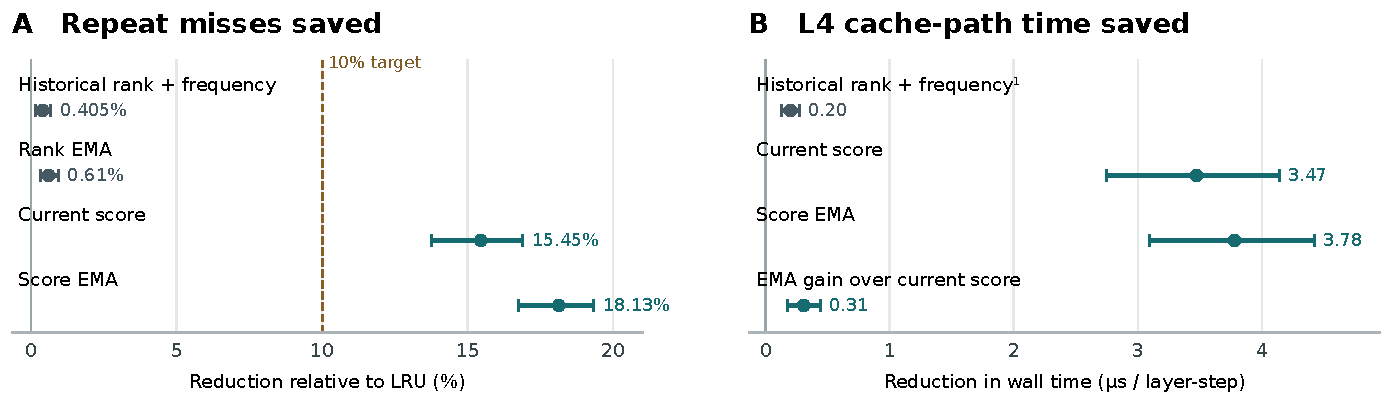
\includegraphics[width=\linewidth]{main_figure.pdf}
\caption{Held-out replacement and hardware effects at $B=128$. Points show pooled reductions and bars show paired 95\% document-bootstrap intervals (10,000 resamples within task and length strata). Panel A uses LRU repeat misses as the denominator. Panel B measures synchronized wall time against LRU, except for the final row, which compares EMA with current scores. Positive values indicate savings. $^{1}$The historical policy used its own paired LRU run.}
\label{fig:kv-main-results}
\end{figure}

\paragraph{Most of the measured L4 gain came from current scores.}
We timed the single-layer cache path with the selection and scores already on the GPU, using cold cache resets and three interleaved wall-time repetitions. The original rank-plus-frequency policy saved 0.202~$\mu$s per layer-step (0.17\%) in its paired benchmark. In the score benchmark, mean times were 125.603~$\mu$s for LRU, 122.130 for current scores, and 121.822 for score EMA. EMA saved 29,441 transfers relative to LRU, or 7.59\% of all transferred pages once first requests are included. Wall time fell by 3.781~$\mu$s (3.01\%, CI for time saved 3.096--4.422). EMA's incremental saving over current scores was 0.308~$\mu$s (0.25\%, CI 0.177--0.443), with lower time on 27 of 40 documents. In separate instrumented runs, the FP64 EMA resolver cost 2.247~$\mu$s more than the current-score resolver, while host packing and H2D copy together saved 0.510~$\mu$s. These components only partially cover the synchronized path, which also includes descriptor return and slot writes. The wall-time comparison establishes the net gain for this implementation. Attributing the entire difference to transfer time would require finer measurements. End-to-end decoding speed remains unmeasured for this short-trace score experiment.
